\chapter{Project Planning and Budget}
\label{ch:planning}

This chapter documents how the project was planned and resourced. It sets out the
development methodology, decomposes the work into a structured breakdown, presents
the thirty-week schedule as a Gantt chart with explicit milestones, assigns
responsibility across the team, records the risks that were identified and how they
were mitigated, and closes with the project budget. A recurring theme throughout is
that the schedule and the budget were shaped by the same constraint that shaped the
architecture: the system had to be buildable and runnable on free-tier hardware with
no paid inference service.

\section{Development Methodology}
\label{sec:plan-method}

The project followed an \emph{incremental, artifact-driven} methodology rather
than a strict waterfall or a fixed-sprint agile process. This choice was
forced by the nature of the system. LectureAssist is a pipeline in which each
stage consumes the output of the previous one, and several of those stages,
optical character recognition, speech transcription, bulk question generation,
are expensive enough that they cannot be re-run casually on a free-tier GPU.
The pipeline was therefore built stage by stage, and each stage was required
to emit a \emph{durable, inspectable artifact} to persistent storage before
the next stage was started.

Three consequences followed from that decision, and all three shaped the schedule
visible in Section~\ref{sec:plan-gantt}.

\paragraph{Stages could be developed and debugged independently.} Because the OCR
stage writes a cached, hashed transcript of every board state to disk, the retrieval
stage could be developed against that cached file without re-running OCR even once.
This is why the extraction tasks and the retrieval task overlap in the schedule
rather than running strictly in series.

\paragraph{Expensive work became resumable.} A Colab runtime disconnection is not an
exceptional event on the free tier; it is a routine one. Checkpointing every
generation and judging run to Google Drive converted a class of failure that would
otherwise have cost days of re-computation into one that costs minutes. Without this,
the bulk evaluation task in weeks 24--27 would not have been feasible at all inside
the schedule.

\paragraph{Measurement was decoupled from generation.} Generation and scoring were
deliberately implemented as separate programs communicating through a JSON artifact
on disk. This meant the evaluation harnesses could be written, corrected and re-run
against an already-generated corpus without regenerating a single question, which
is precisely what happened when the first EQGBench protocol implementation was
judged unfaithful to the published prompt and had to be rewritten.

\section{Work Breakdown Structure}
\label{sec:plan-wbs}

The project was decomposed into five phases containing twenty work packages. Phases
correspond to coherent subsystems rather than to calendar periods, which is why they
overlap in time. Table~\ref{tab:wbs} lists them with their deliverables.

{\footnotesize\singlespacing
\setlength{\tabcolsep}{4pt}
\begin{longtable}{|l|p{5.0cm}|p{5.6cm}|c|}
\caption{Work breakdown structure. Each work package produces a deliverable that a
later package consumes.}
\label{tab:wbs}\\
\hline
\textbf{WP} & \textbf{Work package} & \textbf{Deliverable} & \textbf{Weeks} \\
\hline
\endfirsthead
\hline
\textbf{WP} & \textbf{Work package} & \textbf{Deliverable} & \textbf{Weeks} \\
\hline
\endhead
\hline
\endfoot
\hline
\endlastfoot

\multicolumn{4}{|l|}{\emph{Phase 1, Planning and Research}} \\
\hline
1.1 & Literature review & Annotated bibliography; research gap & 1--5 \\
1.2 & Requirement analysis and scope & Functional requirement list & 2--4 \\
1.3 & Toolchain selection, environment setup & Working Colab + Ollama runtime & 4--6 \\
\hline
\multicolumn{4}{|l|}{\emph{Phase 2, Multimodal Extraction}} \\
\hline
2.1 & Frame sampling and scene classification & Four-class frame router & 5--8 \\
2.2 & Scene-adaptive OCR & Deduplicated board-text blocks & 7--11 \\
2.3 & Speech transcription & Timestamped transcript segments & 8--10 \\
2.4 & Timeline fusion and document parsing & Unified lecture timeline & 10--12 \\
2.5 & Retrieval index construction & FAISS index; \texttt{search\_lecture} tool & 11--13 \\
\hline
\multicolumn{4}{|l|}{\emph{Phase 3, Agentic Generation Pipeline}} \\
\hline
3.1 & Agent framework and orchestrator & \texttt{BaseAgent}; agent event log & 12--15 \\
3.2 & Planner and Generator agents & Topic--difficulty slots; drafted items & 14--17 \\
3.3 & Validator and Refiner loop & Verdict plus remediation action & 16--19 \\
3.4 & Five question types; multi-tier grading & Grading cascade; feedback & 18--21 \\
3.5 & Adaptive difficulty engine & Persistent per-topic profile & 20--22 \\
\hline
\multicolumn{4}{|l|}{\emph{Phase 4, Interface and Integration}} \\
\hline
4.1 & Flask API and tunnel deployment & Public JSON API & 15--18 \\
4.2 & Web interface and live agent workspace & Single-page front end & 17--22 \\
4.3 & End-to-end integration and debugging & Demonstrable system & 21--24 \\
\hline
\multicolumn{4}{|l|}{\emph{Phase 5, Evaluation and Documentation}} \\
\hline
5.1 & Evaluation harnesses & Three scoring programs & 22--26 \\
5.2 & Bulk generation and judging runs & Scored question corpus & 24--27 \\
5.3 & Ablation and merging experiments & Per-agent attribution & 26--28 \\
5.4 & Report, poster and defence & This report; A0 poster & 25--30 \\
\hline
\end{longtable}
}

\section{Project Schedule}
\label{sec:plan-gantt}

Figure~\ref{fig:gantt} presents the thirty-week schedule. The project spans two
academic terms: CSE~499A covers weeks 1--15 and CSE~499B covers weeks 16--30, marked
on the chart by the vertical divider. The division is not merely administrative. By
the end of week 15 the system had to be able to take a lecture video and produce a
grounded, retrievable representation of it; everything that generates, validates or
evaluates questions depends on that representation existing and was therefore
scheduled after it.

\begin{figure}[H]
\centering
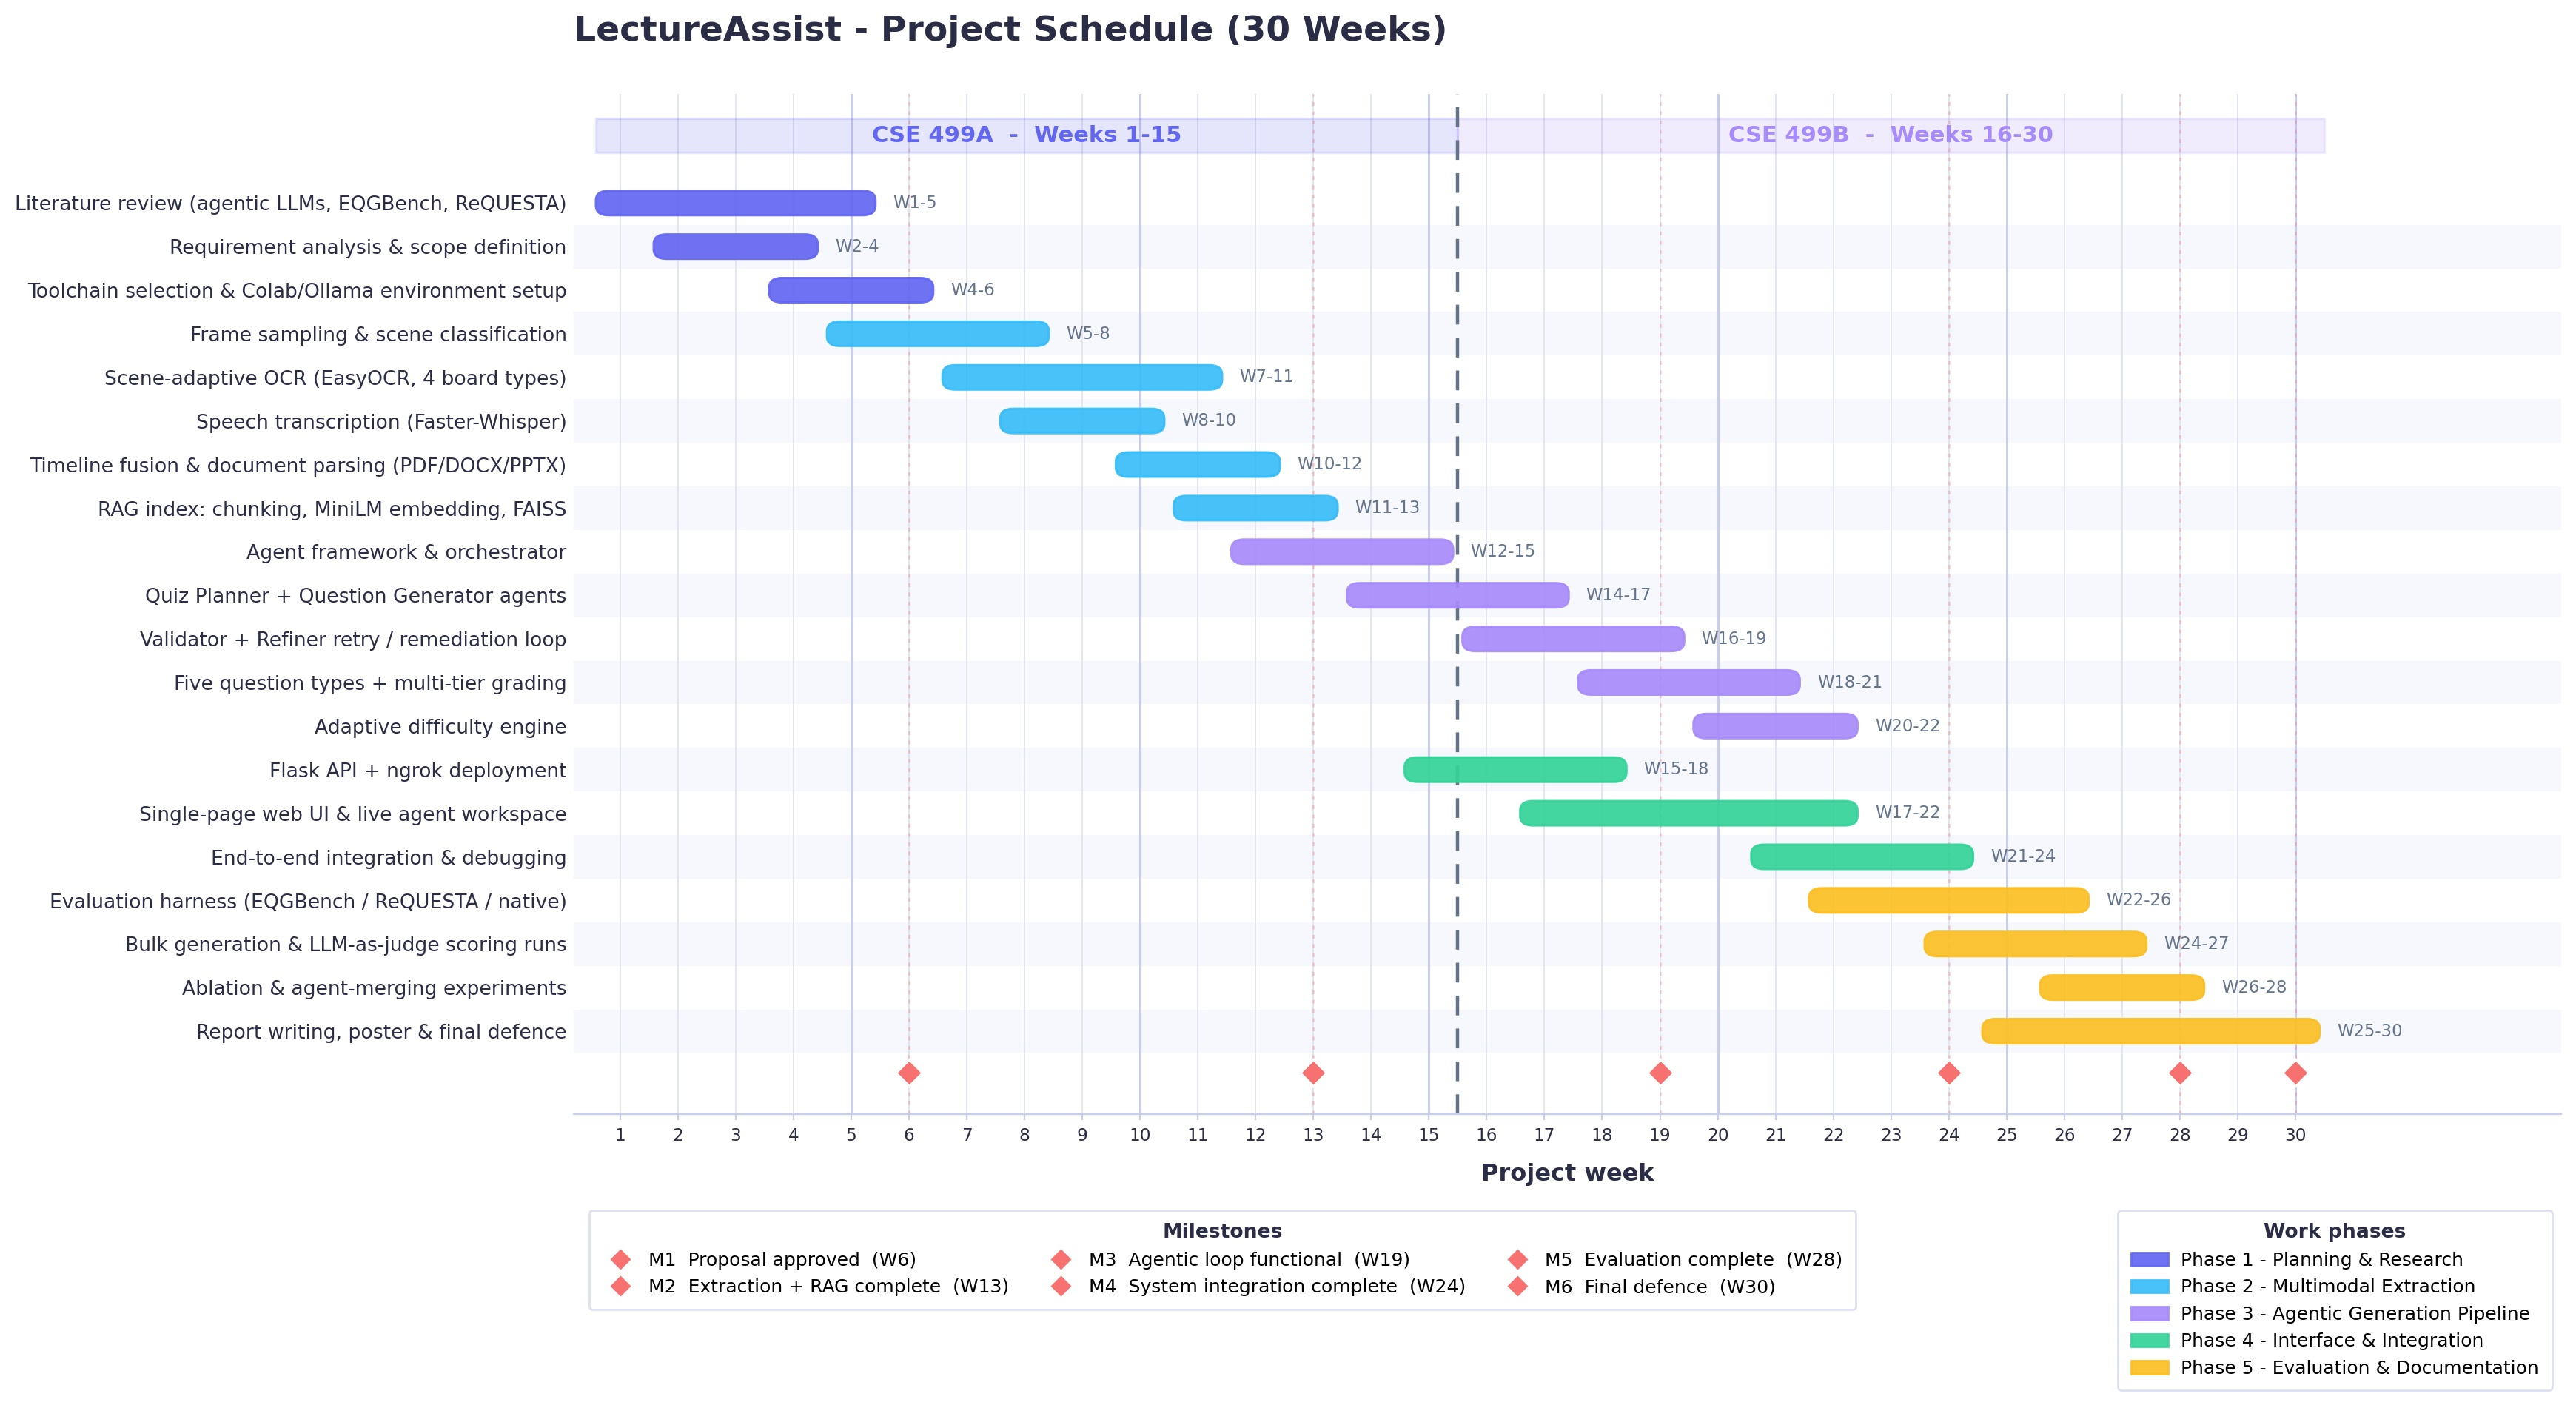
\includegraphics[width=\linewidth]{gantt_chart.jpg}
\caption{Project schedule across thirty weeks, showing twenty work packages grouped
into five phases, the CSE~499A/499B term boundary at week 15, and six milestones.
Overlapping bars reflect the artifact-driven methodology of
Section~\ref{sec:plan-method}: a downstream stage begins as soon as the upstream
stage emits a usable artifact, not when it is finished.}
\label{fig:gantt}
\end{figure}

Three scheduling decisions in that chart are worth justifying explicitly, because
each represents a deliberate trade-off rather than a default.

\paragraph{Extraction and retrieval overlap.} Work package 2.5 begins in week 11,
while OCR work package 2.2 is still running. This was possible only because of the
caching decision described above, and it bought roughly two weeks of slack that were
later consumed by the evaluation phase.

\paragraph{The interface was built early and in parallel.} Front-end work begins in
week 17, well before the pipeline was complete. The reasoning was that the live agent
workspace, which visualises the per-question Plan, Generate, Validate and Retry
trace as it happens, is not merely a presentation layer but a debugging instrument.
Having it available during weeks 18--21 materially accelerated the development of the
validator and refiner, because a failing remediation decision could be seen directly
rather than reconstructed from logs.

\paragraph{Evaluation was given eight weeks, and needed them.} Weeks 22--30 are
dominated by measurement rather than construction. This allocation was made after the
first pilot judging run showed that a faithful implementation of a published protocol
is considerably more work than it appears: EQGBench requires five separate judging
calls per question, repeated over three independent rounds, and ReQUESTA turned out
to publish no judge prompt at all. Both harnesses had to be written from the papers
themselves rather than adapted from released code.

\begin{table}[H]
\centering
\caption{Project milestones and their acceptance criteria.}
\label{tab:milestones}
\footnotesize
\begin{tabular}{|c|c|p{4.2cm}|p{5.4cm}|}
\hline
\textbf{ID} & \textbf{Week} & \textbf{Milestone} & \textbf{Acceptance criterion} \\
\hline
M1 & 6  & Proposal approved &
     Scope, research gap and toolchain agreed with the supervisor \\
M2 & 13 & Extraction and retrieval complete &
     A lecture video yields a fused, timestamped, retrievable timeline \\
M3 & 19 & Agentic loop functional &
     A question is planned, drafted, validated and remediated end to end \\
M4 & 24 & System integration complete &
     All five question types, grading and adaptation reachable from the interface \\
M5 & 28 & Evaluation complete &
     Bulk corpus generated and scored; metrics computed from a real run \\
M6 & 30 & Final defence &
     Report submitted, poster printed, system demonstrated live \\
\hline
\end{tabular}
\end{table}

\section{Team Roles and Responsibilities}
\label{sec:plan-raci}

The team consists of three members working under one supervisor.
Responsibility was assigned per work package using a RACI allocation,
Responsible, Accountable, Consulted, Informed, reproduced in
Table~\ref{tab:raci}. In every row exactly one member is Accountable, so that
no work package could be left un-owned.

{\footnotesize\singlespacing
\setlength{\tabcolsep}{5pt}
\begin{longtable}{|p{5.4cm}|c|c|c|c|}
\caption{RACI responsibility matrix. R = Responsible (does the work),
A = Accountable (owns the outcome), C = Consulted, I = Informed.}
\label{tab:raci}\\
\hline
\textbf{Work package} & \textbf{Iftikhar} & \textbf{Salman} & \textbf{Jarinah}
 & \textbf{Supervisor} \\
\hline
\endfirsthead
\hline
\textbf{Work package} & \textbf{Iftikhar} & \textbf{Salman} & \textbf{Jarinah}
 & \textbf{Supervisor} \\
\hline
\endhead
\hline
\endfoot
\hline
\endlastfoot

Literature review and research gap      & R & C & A & C \\
Requirement analysis and scope          & C & A & R & A \\
Extraction: OCR and scene classification & A & R & C & I \\
Extraction: speech transcription        & R & A & C & I \\
Timeline fusion and document parsing    & A & C & R & I \\
Retrieval index and search tool         & C & A & R & I \\
Agent framework and orchestrator        & R & A & C & C \\
Planner, Generator, Validator, Refiner  & C & A & R & C \\
Question types and grading cascade      & A & R & C & I \\
Adaptive difficulty engine              & R & C & A & I \\
Flask API and deployment                & A & R & I & I \\
Web interface and agent workspace       & R & I & A & I \\
Evaluation harnesses                    & C & A & R & C \\
Bulk runs and result analysis           & R & A & C & C \\
Report, poster and defence              & R & R & R & A \\
\hline
\end{longtable}
}

\section{Risk Management}
\label{sec:plan-risk}

Table~\ref{tab:risks} is the risk register maintained across the project. It is
reproduced here as it was used rather than as a retrospective idealisation, which is
why it includes risks that materialised. Likelihood and impact are rated on a
three-point scale (L/M/H).

{\footnotesize\singlespacing
\setlength{\tabcolsep}{4pt}
\begin{longtable}{|p{3.6cm}|c|c|p{6.4cm}|c|}
\caption{Risk register. Risks marked \emph{occurred} were realised during the
project and were handled by the stated mitigation.}
\label{tab:risks}\\
\hline
\textbf{Risk} & \textbf{L} & \textbf{I} & \textbf{Mitigation} & \textbf{Status} \\
\hline
\endfirsthead
\hline
\textbf{Risk} & \textbf{L} & \textbf{I} & \textbf{Mitigation} & \textbf{Status} \\
\hline
\endhead
\hline
\endfoot
\hline
\endlastfoot

Colab runtime disconnects mid-run &
  H & H &
  Checkpoint every artifact to Drive after each question; make all long runs
  resumable rather than restartable &
  occurred \\
\hline
Free-tier GPU memory insufficient for both the LLM and the embedding model &
  M & H &
  Pin generation to the 4B model; use a 384-dimension embedding model that
  co-exists with it; keep the 12B model for judging only &
  occurred \\
\hline
The 4B generator returns malformed JSON &
  H & M &
  A staged JSON repair chain (escape fixing, quote normalisation, block slicing)
  followed by retry on the same model; never silently escalate to the 12B &
  occurred \\
\hline
Judge API rate limiting stalls the evaluation &
  M & H &
  Row-level checkpointing so a judging run resumes; smoke-test with a small
  sample before committing to a full run &
  occurred \\
\hline
Published protocol cannot be faithfully reproduced &
  M & M &
  Transcribe rubrics directly from the papers; declare every deviation explicitly
  rather than silently approximating &
  occurred \\
\hline
OCR fails on handwritten or low-contrast board work &
  H & M &
  Classify each frame before preprocessing; per-class contrast enhancement and
  polarity inversion; accept that some loss is unavoidable and state it &
  occurred \\
\hline
Team member unavailable during a critical week &
  M & M &
  RACI matrix ensures every package has a named backup in the Responsible column &
  not realised \\
\hline
Scope creep into features not required by the research question &
  M & M &
  Features outside the Plan--Generate--Validate--Refine loop were deferred unless
  they served evaluation or debugging &
  contained \\
\hline
\end{longtable}
}

\section{Budget}
\label{sec:plan-budget}

Figure~\ref{fig:budget} presents the project budget. The total is
$8{,}200$~BDT, approximately USD~$67$ at the conversion rate stated in the figure.

\begin{figure}[H]
\centering
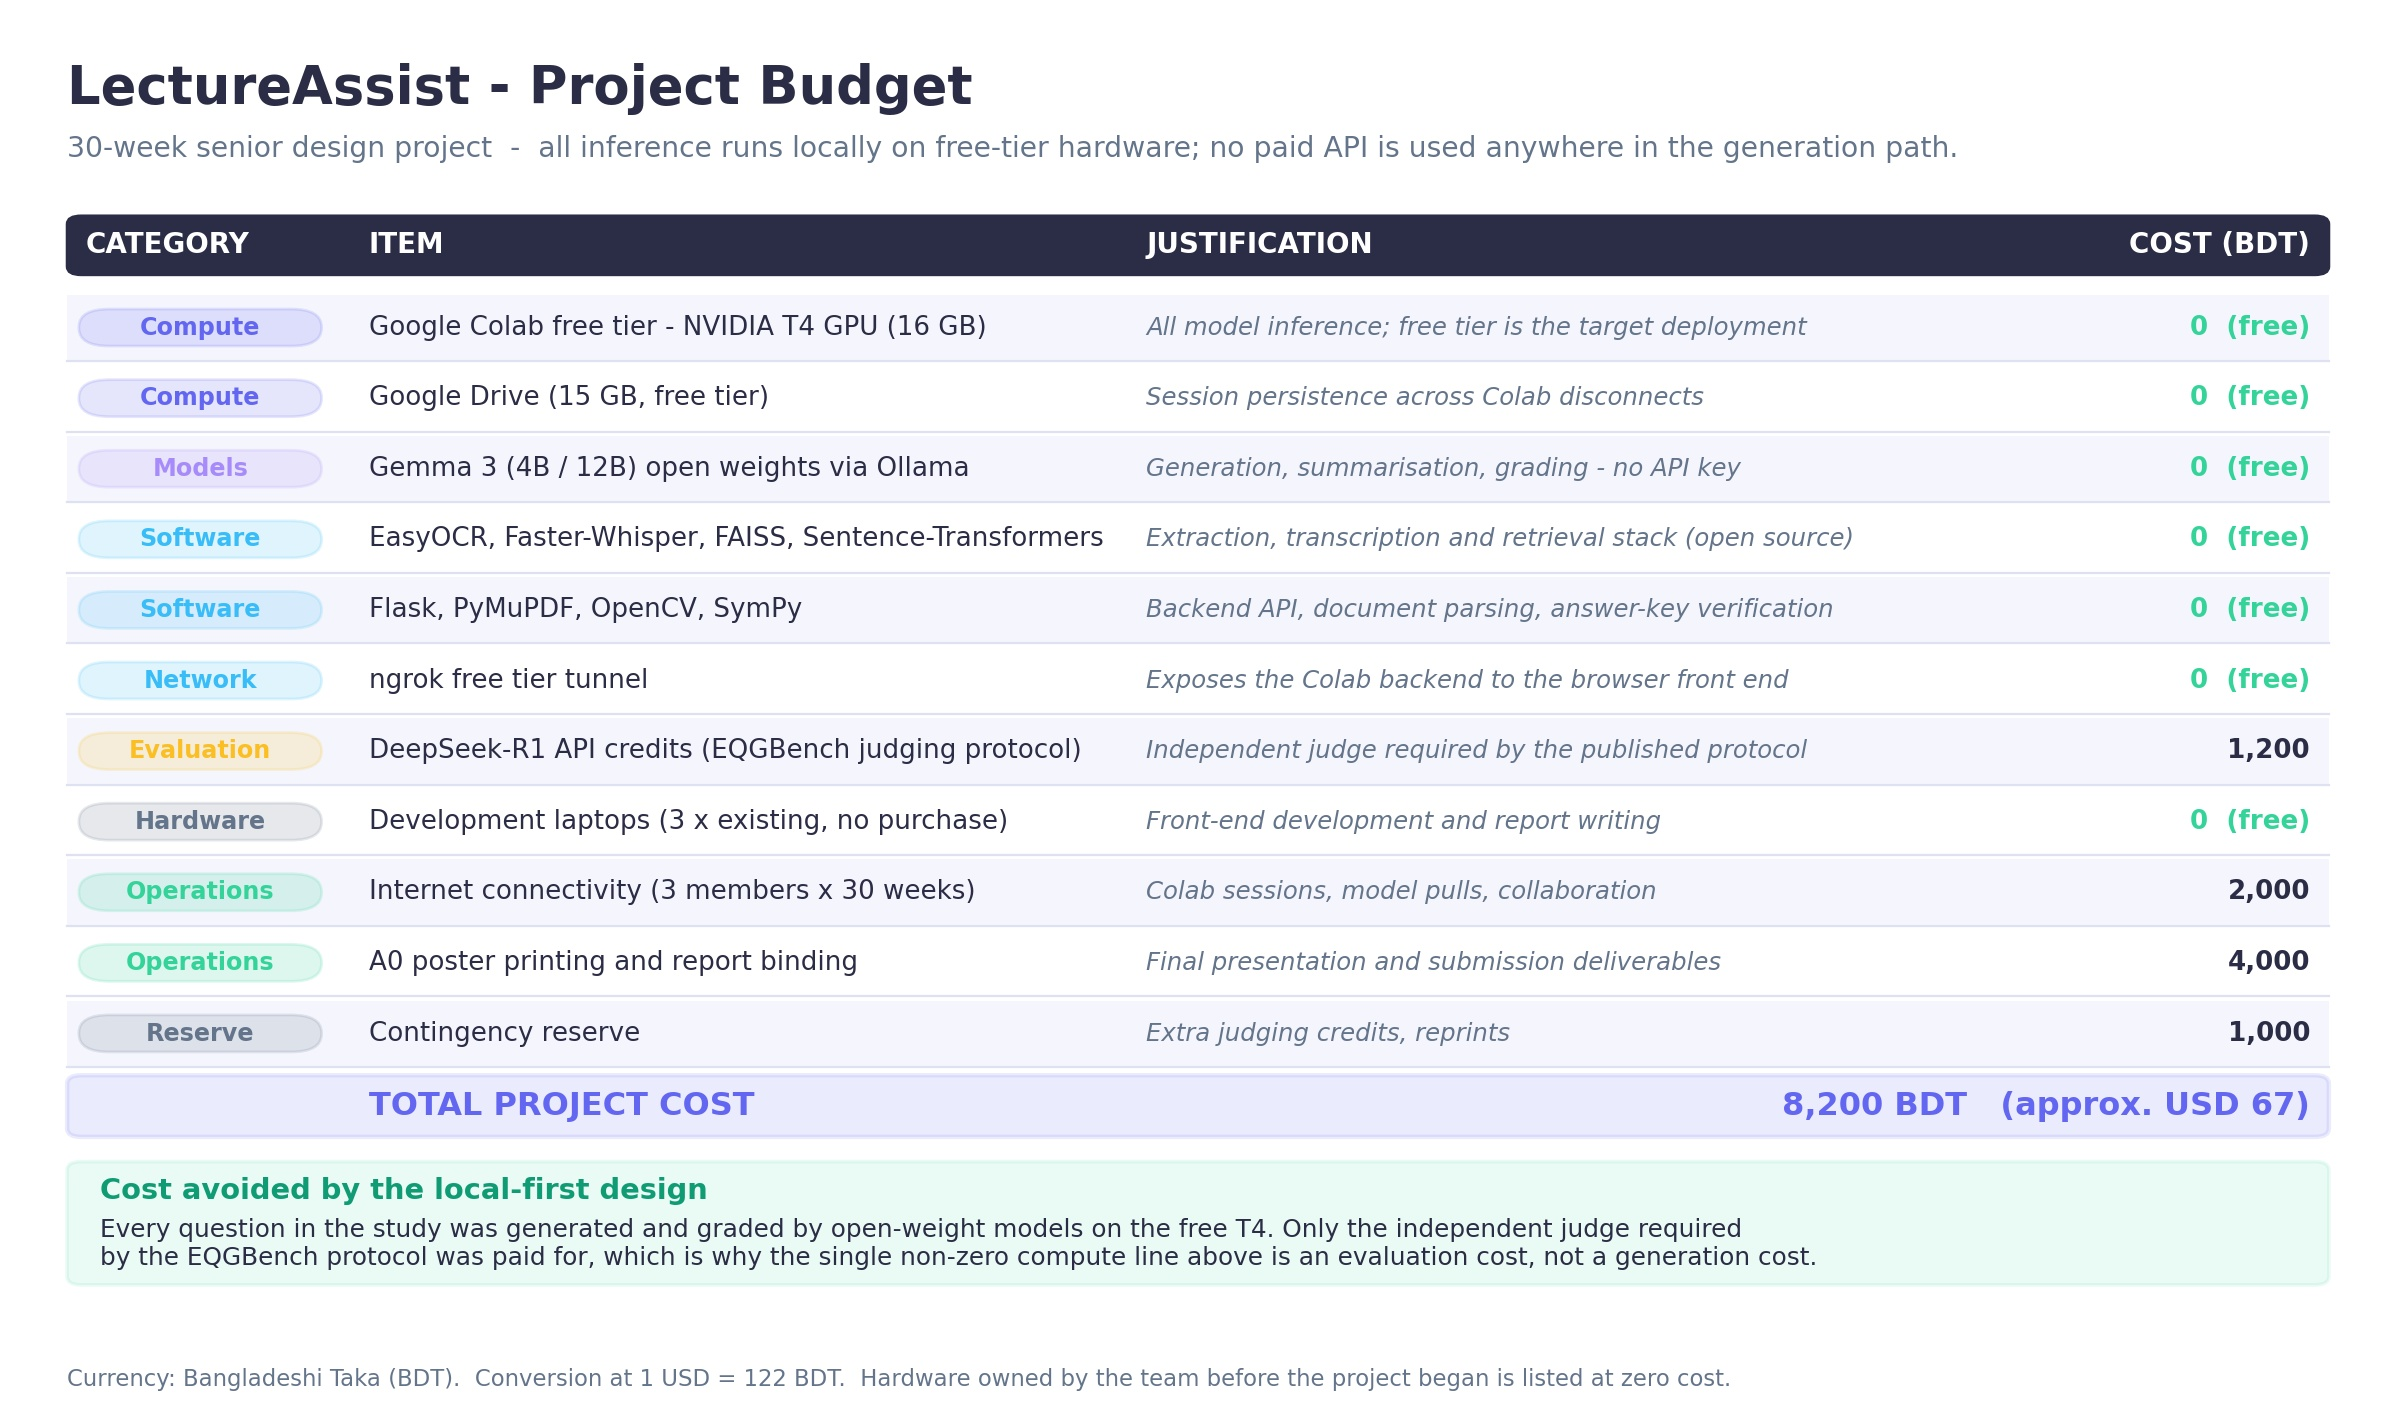
\includegraphics[width=\linewidth]{budget_table.jpg}
\caption{Project budget. Every component on the generation path is free: the compute
is a free-tier NVIDIA T4, the models are open weights served locally, and the
extraction, retrieval and serving stack is open source. The single non-zero technical
line is the independent judge required by the EQGBench protocol, which is an
evaluation cost rather than a system cost.}
\label{fig:budget}
\end{figure}

The structure of that table is the point of it, more than the total. Three
observations follow.

\paragraph{The system itself costs nothing to run.} Every line associated with
producing study material, compute, models, extraction stack, retrieval, serving,
is zero. This is a direct consequence of the constraint stated in
Chapter~\ref{ch:impacts}: a tool whose purpose is to make high-volume retrieval
practice available to students who cannot afford per-token cloud pricing cannot
itself depend on per-token cloud pricing. The engineering cost of that decision is
real and is paid elsewhere in this report: it is why the generator is a $4$B
model, and why so much of Chapter~\ref{ch:methodology} is concerned with extracting
reliable structured output from a small model.

\paragraph{The one paid line is a measurement cost, not a product cost.} EQGBench
specifies DeepSeek-R1 as its judge, and a faithful reproduction of a published
protocol requires using the model the protocol specifies. Substituting a locally
served model would have made the numbers incomparable with the published figures,
which is the entire reason for implementing the protocol faithfully in the first
place. A user of LectureAssist never incurs this cost; only a party reproducing the
evaluation does.

\paragraph{The dominant real cost is human time, which does not appear in the table.}
Roughly $2{,}000$~BDT of the total is connectivity and $4{,}000$~BDT is printing and
binding, so the budget is dominated by overheads that any project of this length
would incur regardless of its subject. The genuine investment in this project was the thirty weeks of work documented
in Section~\ref{sec:plan-gantt}, and the fact that a system of this scope could be
built and evaluated for well under USD~$100$ of direct cost is itself a result worth
recording, since it establishes that the approach is reproducible by any student team
with a laptop and an internet connection.

\paragraph{Cost avoided.} It is worth stating what the alternative would have been.
The evaluation reported in Chapter~\ref{ch:results} involved generating hundreds of
questions per pipeline configuration, each of which consumed multiple LLM calls under
the agentic loop, and then judging every resulting question. Executed against a
commercial frontier API at prevailing per-token rates, that workload would have cost
one to two orders of magnitude more than the entire budget above, and, critically,
it would have made the ablation and merging experiments of
Section~\ref{sec:res-ablation} unaffordable, since those multiply the corpus by the
number of configurations under test. Running locally did not merely save money; it
made a class of experiment possible that would otherwise have been out of reach.
